\documentclass[acmtoms]{acmtrans2m}

\newtheorem{theorem}{Theorem}[section]
\newtheorem{conjecture}[theorem]{Conjecture}
\newtheorem{corollary}[theorem]{Corollary}
\newtheorem{proposition}[theorem]{Proposition}
\newtheorem{lemma}[theorem]{Lemma}
\newdef{definition}[theorem]{Definition}
\newdef{remark}[theorem]{Remark}

\usepackage{amsmath}
\usepackage{amsfonts}
\usepackage{float}
\usepackage{graphicx,wrapfig}
\usepackage{path}
\usepackage{moreverb}
\usepackage{color}

\newcounter{algorithm}
\renewcommand\thealgorithm{\thesection.\arabic{algorithm}}
\newenvironment{algorithm}[2]
{
  \begin{center}
    \noindent
    \framebox{\hbox{
        \begin{minipage}{5in} \refstepcounter{algorithm}
          \vspace{5pt}
          {{\sc Algorithm} \thealgorithm:
            \textsf{\bfseries{#1}} % \hfill \mbox{ ~ }
            } {
            \slshape #2 }
        \end{minipage}
        }}
  \end{center}
  }

%\newcommand{\aspace}[1]{Anasazi::#1}
\newcommand{\aspace}[1]{\texttt{#1}}

\newcommand{\cbcomm}[1]{\textcolor{blue}{\emph{#1}}}
\newcommand{\fin}[1]{\textcolor{red}{\emph{#1}}}

\markboth{C. G. Baker et al}{Anasazi software for the numerical
solution of large-scale eigenvalue problems}

\title{Anasazi software for the numerical solution of large-scale eigenvalue problems}

\author{C. G. Baker and
U. L. Hetmaniuk and R. B. Lehoucq and H. K. Thornquist\\ Sandia
National Laboratories}

\begin{abstract}
Anasazi is a package within the Trilinos software project that
provides a framework for the iterative, numerical solution of 
large-scale eigenvalue problems. Anasazi is written in ANSI C++ and
exploits modern software paradigms to enable the research and development
of eigensolver algorithms. Furthermore, Anasazi provides implementations
for some of the most recent eigensolver methods.
The purpose of our paper is to describe the design and
development of the Anasazi framework. A performance comparison 
of Anasazi and the popular FORTRAN 77 code ARPACK is given. 
\end{abstract}

\category{G.1.3}{Numerical Analysis}{Numerical Linear Algebra}
\category{G.4}{Mathematical Software}{} \category{D.2.13}{Software
Engineering}{Reusable Software}

\terms{Algorithms, Design, Performance; Reliability, Theory}

\keywords{Eigenvalue problems, Numerical Algorithms, Generic
programming, Object-oriented programming, Large-scale scientific computing}

\begin{document}

\begin{bottomstuff}
Sandia is a multiprogram laboratory operated by Sandia Corporation,
a Lockheed Martin Company, for the United States Department of
Energy under contract DE-AC04-94AL85000. Authors' addresses: C. G.
Baker, U. L. Hetmaniuk, R. B. Lehoucq,
Sandia National Laboratories, Computational Mathematics \&
Algorithms, MS 1320, P.O.Box 5800, Albuquerque, NM 87185-1320; email
\{cgbaker,ulhetma,rblehou\}@sandia.gov. H. K. Thornquist, Sandia National
Laboratories, Electrical and Microsystem Modeling, MS 0316,
Albuquerque, NM 87185-0316; email hkthorn@sandia.gov.

\end{bottomstuff}

\maketitle

Anasazi is a package within the Trilinos Project~\cite{Heroux:2005:OTP} that uses ANSI C++
and modern software paradigms to implement algorithms for the numerical solution of
large-scale eigenvalue problems. We define a large-scale eigenvalue problem to be one
where a small number (relative to the dimension of the problem) of eigenvalues and the
associated eigenspace are computed and only knowledge of the underlying matrix via
application on a vector (or group of vectors) is assumed.

An inspiration for Anasazi is the ARPACK~\cite{lesy:98} FORTRAN 77 software library.
ARPACK implements a single algorithm, namely an implicitly restarted Arnoldi
method~\cite{sore:92}. In contrast, Anasazi provides a software framework, including the
necessary infrastructure, to implement a variety of algorithms. We justify our claims by
implementing block variants of three popular algorithms: a Davidson~\cite{morganscott:86} method,
a Krylov-Schur~\cite{stew:01} method, and an implementation of LOBPCG~\cite{knya:01}.

ARPACK has proven to be a popular and successful FORTRAN 77 library for the numerical
solution of large-scale eigenvalue problems. A crucial reason for the popularity of ARPACK
is the use of a reverse communication~\cite[p.~3]{lesy:98} interface for applying the
necessary matrix-vector products. This allows ARPACK to provide a callback for the needed
matrix-vector products in a simple fashion within FORTRAN 77. This flexibility has enabled the use of
ARPACK in a wide range of applications, and it is this flexibility that Anasazi was
designed to emulate.

The design goals of Anasazi were multiple. First, implementation of eigensolvers should be
independent from the choice of underlying linear algebra primitives. The benefit is that
the resulting eigensolvers are able to exploit existing software, such as the wide variety
of linear algebra implementations, solvers, and preconditioners present in Trilinos. This
flexibility also eases the incorporation of Anasazi into larger software libraries and
application codes.

Another goal of Anasazi is that abstract interfaces should be utilized wherever feasible
for algorithmic components, so that the implementation of those components may be
separated from the implementation of the eigensolvers. Many benefits result from such a
decision. This decoupling facilitates code reuse across and outside of the Anasazi
eigensolvers. This underlies Anasazi's existence as a framework for developing novel
eigensolver capability. This decoupling also increases algorithmic flexibility. As a
result, constituent mechanisms (e.g., orthogonalization routines) can be chosen at
runtime. This cements Anasazi's usefulness as a framework for research, not only into
eigensolvers, but also the components necessary to implement an eigensolver.

The Anasazi framework accomplishes these design goals by exploiting more recent software
development paradigms than available to related eigensolver software. Both generic and
object-oriented programming, via static and dynamic polymorphism~\cite[Chapter 14]{VJ02},
are employed to this effect. Static polymorphism, via templating of the linear algebra
primitives, allows algorithms in Anasazi to be written in a generic manner (i.e.,
independent of the data types). Dynamic polymorphism, via virtual functions and
inheritance, allows eigensolvers to be decoupled from constituent mechanisms such as
orthogonalization and stopping conditions. 

We emphasize that our interest is not solely in modern software paradigms. Rather, our
paper demonstrates that a rich collection of efficient block eigensolvers is easily
implemented using modern programming techniques. Our approach is algorithm-oriented
\cite{muov:94}, in that requirements for efficient implementation of the necessary
algorithms were considered first. This was followed by a formulation of the software
abstractions capable of implementing these algorithms, and their constituent mechanisms,
in sufficiently diverse ways. The result was a collection of implementations that are both
efficient and flexible. 

The purpose of this paper is to introduce the Anasazi software framework to prospective
users. These users include practitioners and researchers in need of efficient, large-scale
eigensolvers. This also includes experts who could exploit the framework provided by
Anasazi as a platform for research and development of new methods for solving eigenvalue
problems. This paper is intended to outline the benefits of Anasazi's design, as well as
the motivation for those decisions. More in-depth documentation is available at the
project webpage~\cite{Trilinos:Anasazi}.

\section{Related eigensolver software}
%%%%%%%%%%%%%%%%%%%%%%%%%%%%%%%%%%%%%%%%%%%%%%%%%%%%%%
\label{sec:related-software}

There exist a number of related software efforts for solving large-scale eigenvalue problems (the
reader is referred to~\cite{slepc:05} for a more complete survey). We discuss here the
ARPACK, IETL, PRIMME and SLEPc software efforts:
\begin{itemize}
  \item 
    The Arnoldi Package (ARPACK) is a FORTRAN 77 software for the solution of Hermitian or
    non-Hermitian, standard or generalized, eigenvalue problems. ARPACK implements a single
    solver, the Implicitly Restarted Arnoldi Method.
  \item 
    The Iterative Eigensolver Template Library (IETL) is a C++ library which uses C++
    templates to provide a collection of generic eigensolvers. It currently provides four
    solvers for standard Hermitian eigenvalue problems.
  \item
    The Preconditioned Iterative Multi-Method Eigensolver (PRIMME)~\cite{primme:06} is a C
    library for computing a number of eigenvalues and the corresponding eigenvectors of a real
    symmetric or complex Hermitian matrix. PRIMME provides a highly parametrized
    Jacobi-Davidson~\cite{slvo:96} iteration, allowing the behavior of multiple eigensolvers
    to be obtained via the appropriate selection of parameters.
  \item
    The Scalable Library for Eigenvalue Problem Computations (SLEPc)~\cite{slepc:06} library
    is another C library for the solution of large scale sparse eigenvalue problems on parallel
    computers. SLEPc is an extension of the popular PETSc~\cite{petsc-web-page} and can be
    used for either Hermitian or non-Hermitian, standard or generalized, eigenproblems.
\end{itemize}

ARPACK utilizes a reverse-communication interface to access the linear operators defining
the eigenvalue problem. As a result, the eigensolver is implemented in a partially generic
manner, independent of the underlying linear operator, allowing use of the software for
many user-defined eigenproblems. A more recent effort (PARPACK) extends ARPACK to provides
a parallel computing capability. These reasons, along with ARPACK's maturity, make it the
\textit{de facto} eigensolver in many scientific computing communities. Unfortunately, the
reverse communication interface makes maintenance of ARPACK a cumbersome task.
Furthermore, while this interface does provide a generic interface for the linear
operators, the storage of vector data is fixed. In addition to limiting any flexibility in
data representation, this fixed interface results in software which is susceptible to any
(albeit unlikely) design changes in ARPACK.

The IETL software library, like ARPACK, strives to ease use of the software in diverse
applications through a generic interface to operators and vectors. Implemented in C++,
IETL achieves this through the language's template feature. By utilizing generic
interfaces for scalar types, vectors and linear operators, IETL solvers can be applied to
any data structures which adhere to the prescribed object model. This allows a single
implementation of an eigensolver in IETL to be exploited across many different programming
environments, e.g., real or complex arithmetic, parallel or serial architecture.

PRIMME provides a flexible metasolver capable of implementing a variety of Hermitian
eigensolvers. Packaged parameter choices are provided to emulate a number of popular
eigensolvers, allowing easy use of the software by novice users. Expert users may manually
specify the parameters in order to access the full flexibility available in the solver's
behavior. Therefore, PRIMME is valuable both as a convenient eigensolver for practitioners
and a platform for experimentation by eigensolver researchers. However, while parameters
are provided to control mechanisms such as, e.g., stopping conditions and
orthogonalization, the user is limited to the implementations provided by the developers
of PRIMME. As a result, the extensibility of the solver is limited to those options
anticipated by the developers. Furthermore, PRIMME provides implementations only over
double precision real and complex fields. Each additional scalar field (such as
\texttt{float} or extended precision) requires a separate implementation, due to the lack
of generic programming ability in the C programming language.

SLEPc extends the PETSc toolkit to provide a library of solvers for standard or
generalized, Hermitian or non-Hermitian eigenproblems. SLEPc provides wrappers for several
eigensolver packages, most notably ARPACK and PRIMME, as well as native implementations of
eigensolvers like Krylov-Schur, Arnoldi, and Lanczos. PETSc uses C language features such
as \texttt{typedef}s and function pointers to support some generic programming and
object-oriented programming techniques, the goal being interoperability with other
software packages. Interoperability with PETSc gives SLEPc users access to a large library
of linear and nonlinear solvers, preconditioners and matrix formats, though SLEPc's
reliance on PETSc requires that users employ PETSc for vector storage. Similar to PRIMME,
SLEPc can be compiled with support for double precision real or complex arithmetic.
However, only one version of the library can be used at a time. Furthermore, mechanisms
such as orthogonalization are hard-coded, allowing only parametrized control over their
behavior. 

The Anasazi framework was designed to include features from other eigensolver packages
that are conducive to algorithm development, while avoiding some of the drawbacks
mentioned above. The most important features that have been incorporated into its design
are extensibility and interoperability. The extensibility of the Anasazi framework is
demonstrated through the infrastructure's support for a significant class of large-scale
eigenvalue algorithms. Extensions can be made through the addition of, or modification to,
existing algorithms and auxiliary functionality such as orthogonalization, desired
eigenvalue selection, and stopping conditions. This is encouraged by promoting code
modularization and multiple levels of access to solvers and their data.  The question of
whether to implement a new solver in PRIMME is a question of whether the PRIMME metasolver
is capable of describing the desired solver without excessive modification. For libraries
such as SLEPc and IETL, this decision is made based largely on the existing functionality
that can be exploited in the library. By decoupling eigensolvers from constituent
mechanisms, Anasazi allows such functionality to be exploited by new solvers. This design
also allows new implementations of this functionality to be exploited by existing
eigensolvers. This is the foundation of extensibility in Anasazi.

Interoperability in the Anasazi framework is enabled via the treatment of both matrices
and vectors as opaque objects---only knowledge of the matrix and vectors via elementary
operations is necessary. This permits algorithms to be implemented in a generic manner,
requiring no knowledge of the underlying linear algebra types or their specific
implementations. Furthermore, the Anasazi framework was designed to admit operation with
any user choice of scalar field, vector and operator. This is accomplished using the
template mechanism in the C++ programming language, an option not available to SLEPc or
PRIMME. As a result, for example, an Anasazi eigensolver using single-precision complex
arithmetic can be used alongside another Anasazi eigensolver using an extended precision
scalar type; both are instantiated from the same source code.

As a result of these design features, the Anasazi eigensolver framework is significantly
more flexible than previous efforts, allowing its inclusion in diverse application
environments in addition to providing an arena for research into eigensolvers and their
constituent mechanisms. The rest of this paper is organized as follows.
Section~\ref{sec:algorithm-overview} briefly discusses one class of algorithms that can be
implemented using Anasazi, in order to explore the types of operations necessary for an
eigensolver framework. Section~\ref{sec:framework} reviews the Anasazi framework,
discusses some of the design decisions, and illustrates the benefits of these decisions.
Lastly, Section~\ref{sec:benchmarking} provides some timings comparing ARPACK and Anasazi
to demonstrate that object-oriented overhead has no impact on the performance of this
modern software framework.


\section{Algorithmic Inspiration}
%%%%%%%%%%%%%%%%%%%%%%%%%%%%%%%%%%%%%%%%%%%%%%%%%%%%%%
\label{sec:algorithm-overview}

The Anasazi software framework provides tools that are useful for solving a wide variety
of eigenvalue problems. While development of the package continues to expand its scope to
other important eigenvalue problems (e.g., nonlinear eigenproblems, constrained
eigenproblems), the solvers currently released with the package are aimed at computing a
partial eigen-decomposition for the generalized eigenvalue problem
\begin{equation}  \label{eq:intro.1}
  \mathbf{A} \mathbf{x} = \mathbf{B} \mathbf{x} \lambda , \qquad
  \mathbf{A}, \mathbf{B} \in \mathbb{C}^{n\times n}\ .
\end{equation}
In this paper, the matrices $\mathbf{A}$ and $\mathbf{B}$ are large, possibly sparse, and
we assume that only their application to a block of vectors is required. The reader is
referred to~\cite{saad:92,sore:02,stew:01book,vors:02} for background information and
references on the large-scale eigenvalue problem.

% \begin{figure}[htb]
% \begin{algorithm}{Rayleigh-Ritz Algorithm\label{algo:obliqueRR}}
% {\smallskip
% \begin{tabbing}
% (nr)ss\=ijkl\=bbb\=ccc\=ddd\= \kill {\rm (1)} \>\> Let the matrix
% $\mathbf{M}$ and bases $\mathbf{U}$, $\mathbf{V}$ be given
% \\
% {\rm (2)} \>\> Form the Rayleigh quotients $ \mathbf{V}^H
% \mathbf{M}\mathbf{\Phi}(\mathbf{A}) \mathbf{U}$ and $ \mathbf{V}^H \mathbf{M}
% \mathbf{\Psi}(\mathbf{B}) \mathbf{U}$\\
% \>\> where $\mathbf{\Phi}(\cdot)$ and $\mathbf{\Psi}(\cdot)$ are matrix functions
% \\
% {\rm (3)} \>\> Compute an eigen-decomposition $(\mathbf{L},\mathbf{W})$ for the Rayleigh
% quotients\\
% \>\>\>\>$ \left(\mathbf{V}^H \mathbf{M}\mathbf{\Phi}(\mathbf{A}) \mathbf{U}\right) \mathbf{W} = 
% \left(\mathbf{V}^H \mathbf{M}\mathbf{\Psi}(\mathbf{B}) \mathbf{U}\right) \mathbf{W} \mathbf{L}$
% \\
% {\rm (4)} \>\> Use the decomposition $(\mathbf{L},\mathbf{W})$ and the basis $\mathbf{U}$
% to construct \\
% \>\>approximate eigenpairs for the pencil $(\mathbf{A}, \mathbf{B})$
% \\
% \end{tabbing}
% }
% \end{algorithm}
% \end{figure}

\begin{figure}[htb]
\begin{algorithm}{Block Davidson Algorithm\label{algo:blockdavid}}
{\smallskip
\begin{tabbing}
(nr)ss\=ijkl\=bbb\=ccc\=ddd\= \kill 
{\rm (0)} \> Initial $\mathbf{B}$-orthonormal basis $\mathbf{V}_0$ \\
          \> for $i=1,\ldots$ \\
{\rm (1)} \>\> Project $\mathbf{A}$ onto $\mathbf{V}_{i-1}$: \\
          \>\>\>\> $\mathbf{\hat{A}} = \mathbf{V}_{i-1}^H A \mathbf{V}_{i-1}$ \\
{\rm (2)} \>\> Compute select eigenpairs $\mathbf{Q}$, $\mathbf{\Gamma}$ of $\hat{A}$: \\
          \>\>\>\> $\mathbf{\hat{A}} \mathbf{Q} = \mathbf{Q} \mathbf{\Gamma}$ \\
{\rm (3)} \>\> Compute Ritz vectors: \\
          \>\>\>\> $\mathbf{X} = \mathbf{V}_{i-1} \mathbf{Q}$ \\ 
          \>\> and residuals: \\
          \>\>\>\> $\mathbf{R} = \mathbf{A} \mathbf{X} - \mathbf{B} \mathbf{X} \mathbf{\Gamma}$ \\
{\rm (4)} \>\> Precondition the residuals: \\
          \>\>\>\> $\mathbf{H} = \mathbf{P}\mathbf{R}$ \\
{\rm (5)} \>\> Check convergence and possibly terminate iteration. \\
{\rm (6)} \>\> Compute $\mathbf{B}$-orthonormal basis $\mathbf{V}_i$ for $\begin{bmatrix} \mathbf{V}_{i-1} & H \end{bmatrix}$ \\
          \> endfor
\end{tabbing}
}
\end{algorithm}
\end{figure}

Algorithm~\ref{algo:blockdavid} is a simple description of the block Davidson eigensolver
provided by Anasazi and described in~\cite{Arbenz:2005:ACE}.  This algorithm lists the
salient steps found in the majority of large-scale eigensolvers, namely subspace
projection methods.  The linear operators $\mathbf{A}$ and $\mathbf{B}$ define the
eigenproblem to be solved, and the linear operator $\mathbf{N}$ is a preconditioner for
the problem.  The matrix $\mathbf{V}$ is the basis for the Rayleigh-Ritz approximation
conducted at each step, and here it is required to be orthonormal with respect to the
inner product induced by the Hermitian positive-definite matrix $\mathbf{B}$.

The block Davidson eigensolver as described above is useful for examining some of the
functionality that should be provided by a general eigensolver framework. However, first
we should observe some general structure of the participants in this algorithm. The basis
$\mathbf{V}$ and the matrices $\mathbf{X}$ and $\mathbf{R}$ are dense matrices that are
stored as a collection of vectors, which we call a \emph{multivector}. Interaction with
$\mathbf{A}$, $\mathbf{B}$, and $\mathbf{N}$ requires knowledge of the underlying matrix
via application on a vector or multivector. Thus we regard these matrices as
\emph{operators}.

Given these observations, the functionality that is important to an eigensolver includes:
\begin{itemize}
  \item multivector creation: create $\mathbf{V}$, $\mathbf{X}$
  \item operator-multivector applications: $\mathbf{A} X$, $\mathbf{N} R$;
  \item multivector arithmetic: $\mathbf{X}^H \mathbf{Y}$;
  \item solution of typically much smaller eigenproblems (step~2).
\end{itemize}
A full list of our primitives for operators and multivectors will be presented in Section \ref{sec:framework}. 
It is worthwhile to note at this point that the Anasazi framework was designed to support block methods,
defined as those that apply $\mathbf{A}$ or $\mathbf{B}$ to a collection of vectors, or multivector.
One advantage of using a multivector data structure is to improve the ratio of 
floating-point operations to memory references and so better exploit a memory hierarchy.

Algorithm~\ref{algo:blockdavid} needs to be augmented with several details in order to
result in a complete implementation. The decisions involved in Steps~2 and 5 require a
determination of the interesting portion of the eigen-decomposition and a definition of
accuracy or algorithmic breakdown, thus they are likely candidates for decoupling from the
implementation of a particular eigen-iteration. Steps~0 and 6, whatever their
implementation, will require some methods for orthogonalization/orthonormalization, which
are an active area of research. After a certain number of iterations, it may be worthwhile
to terminate the iteration and restart with a smaller basis, in order to limit the amount
of memory required and the computation expended. The restarting of this eigensolver can be
performed in a variety of ways and therefore need not be tightly coupled to the
eigensolver. Each of these mechanisms provide opportunity for decoupling functionality
that need not be implemented in a specific manner. 

This discussion illustrates that many distinct parts make up a large-scale eigensolver
code: orthogonalization, sorting tools, dense linear algebra, convergence testing,
multivector arithmetic, etc. Anasazi presents a framework of algorithmic components,
decoupling operations where possible in order to simplify component verification,
encourage code reuse, and maximize flexibility in implementation.


\section{Anasazi software framework}
%%%%%%%%%%%%%%%%%%%%%%%%%%%%%%%%%%%%%%%%%%%%%%%%%%%%%%
\label{sec:framework}

This section outlines the Anasazi software framework and discusses 
the design decisions made in the development of Anasazi. Three
subsections describe the Anasazi operator/multivector interface, the
eigensolver framework, and the various implementations provided by the
Anasazi framework. The reader is referred to
\cite{Trilinos:Anasazi,Trilinos-Tutorial} for software documentation
and a tutorial.

We remark that Anasazi is largely independent of other Trilinos packages and
third-party libraries. However, Anasazi does rely on the Trilinos Teuchos 
package~\cite{Trilinos:Teuchos} to provide tools, such as: \texttt{RCP},
a reference-counting smart pointer~\cite{Detlefs:1992:GCR,Teuchos-RCP};
\texttt{ParameterList}, a list for algorithmic parameters of
varying data types; and the BLAS \cite{Lawson:1979:BLA,Blackford:2002:USB} 
and LAPACK \cite{abbd:95} C++ wrappers.
The only third-party libraries that Anasazi requires are the BLAS and
LAPACK libraries, which are essential in performing the dense arithmetic
for Rayleigh-Ritz methods.

%In order to perform the Rayleigh-Ritz analysis used by the
%algorithms illustrating this section, Anasazi utilizes the classes
%\aspace{Teuchos::BLAS} and \aspace{Teuchos::LAPACK}. The purpose of
%these classes is to provide templated interfaces to the dense linear
%algebra routines provided by the BLAS and LAPACK libraries.
%Therefore, even such operations as dense matrix-matrix
%multiplication are made independent of the scalar field defining the
%eigenvalue problem. Users are therefore currently limited to
%algorithms provided by LAPACK.

\subsection{The Anasazi Operator/Multivector Interface}
%%%%%%%%%%%%%%%%%%%%%%%%%%%%%%%%%%%%%%%%%%%%%%%%%%%%%%
\label{sec:anasazi:opvec}

Anasazi utilizes traits classes~\cite{myer:95,veld:96} to define interfaces for the scalar field,
multivectors, and matrix operators. This allows generic programming techniques to
be used when developing numerical algorithms in the Anasazi framework.  
Anasazi's eigensolver framework (Section  
\ref{subsec:anasazi:solver_framework}) is comprised of abstract numerical interfaces
that are all implemented using templates and the functionality of the 
template arguments is provided through their corresponding trait classes.
Most classes in Anasazi accept
three template parameters:
\begin{itemize}
\item
a scalar type, describing the field over which the vectors and
operators are defined;
\item
a multivector type over the given scalar field, providing a
data structure that denotes a collection of vectors; and
\item
an operator type over the given scalar field,
providing linear operators used to define eigenproblems and
preconditioners.
\end{itemize}

Templating an eigensolver on operator, multivector, and scalar types makes software reuse
easier. Consider in contrast that ARPACK implements the subroutines \texttt{SNAUPD},
\texttt{DNAUPD}, \texttt{CNAUPD}, and \texttt{ZNAUPD} for solving non-Hermitian
eigenproblems. Separate subroutines are required for each of the four FORTRAN 77 floating
point types (single and double precision real, and single and double precision complex).
Moreover, four additional subroutines are needed for a distributed memory implementation.
By templating abstract numerical interfaces on operator, multivector, and scalar types, 
it is only necessary to maintain a single code using the Anasazi framework.

\begin{figure}[htb]
\label{fig:latemplate}
\begin{center}
%\includegraphics[height=1.5in]{interface_level5}
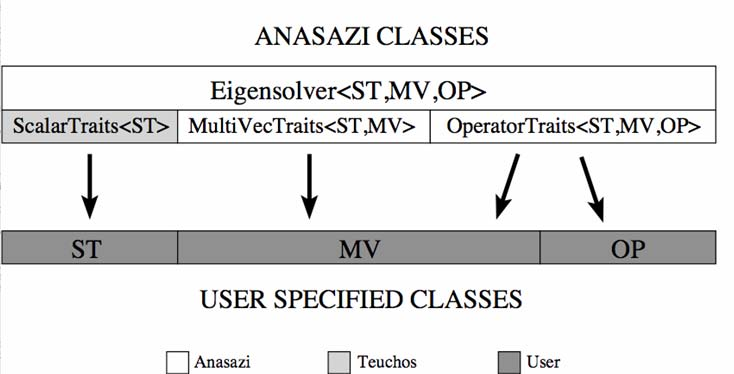
\includegraphics[height=1.5in]{anasazi_linalg_template}
\end{center}
\caption{An eigensolver templated on scalar (ST), multivector (MV), and
operator (OP) type.}
\end{figure}

Another aspect of software reuse that templating alleviates is through the separation of the
eigensolver algorithm from the linear algebra data structures.  This separation, as shown in
Figure \ref{fig:latemplate}, allows a user of the Anasazi framework to leverage an existing 
linear algebra software investment.  All that is required is the template instantiation of the trait
classes, \aspace{MultiVecTraits} and \aspace{OperatorTraits}, for the user-defined multivector 
and operator, respectively.  The \aspace{ScalarTraits} class and respective template 
instantiations for different scalar types are provided by the Trilinos Teuchos package 
\cite{Trilinos:Teuchos}. Another friendly aspect of employing templates and traits mechanisms
is that the Anasazi eigensolver, eigenproblem, and eigensolution are all defined by the 
specified scalar, multivector, and operator type at compile time.  This approach, as opposed to
using abstract interfaces and dynamic polymorphism, avoids any dynamic casting of the multivectors 
and operators in the user's interaction with the Anasazi framework.

%eigenvalue algorithm from the linear algebra data structures. The operator type templating
%is analogous to the reverse communication interface used by ARPACK for providing
%matrix-vector products.

%Because the underlying data types are unknown to the Anasazi
%developer, algorithms are developed abstractly. Access to the
%functionality of the underlying objects is provided via the classes
%\aspace{MultiVecTraits} and \aspace{OperatorTraits}. These classes
%implement the traits mechanism~\cite{myer:95} and specify the
%operations that the multivector and operator classes must support in
%order to be used within Anasazi. This mechanism hides the low-level
%details of the underlying data structures.  As a result, a single
%eigensolver implementation in Anasazi can be exploited on a number of
%diverse computing platforms: serial, distributed memory parallel,
%multi-core shared memory parallel, graphics processing units, FPGAs,
%etc.

The \aspace{MultiVecTraits} and \aspace{OperatorTraits} classes specify
the operations that the multivector and operator type must support in order for them to be
used by Anasazi. Through the observations made in Section \ref{sec:algorithm-overview}, 
it is clear that the \aspace{OperatorTraits} class only needs to provide one method,
described in Table \ref{tab:anasazi:opt}, that applies an operator to a multivector.  
This interface defines the only interaction required from an operator, even though
the underlying operator may be a matrix, 
spectral transformation, or preconditioner.
\begin{table}[bth]
\begin{center}
  \caption{The method provided by the \aspace{OperatorTraits} interface.}
\label{tab:anasazi:opt}
\begin{tabular}{| p{4cm} | p{8cm} |}
\hline
%%
\multicolumn{2}{|c|}{\textbf{OperatorTraits$<$ST,MV,OP$>$}} \\\hline
\emph{Method name} & \emph{Description} \\\hline
{\tt Apply(A,X,Y)} & Applies the operator $A$ to the multivector $X$, placing the
result in the multivector $Y$ \\
\hline
%%
\end{tabular}
\end{center}
\end{table}

The methods defined by the \aspace{MultiVecTraits} class, listed in
Table~\ref{tab:anasazi:mvt}, are the creational and arithmetic methods necessitated
by the observations in Section \ref{sec:algorithm-overview}.
The creational methods generate empty or populated multivectors from a previously
created multivector. The populated multivectors can be 
a deep copy, where the object contains the storage for the multivector entries, or a shallow copy, 
where the object has a view of another multivector's storage.
A shallow copy is useful when only a
subset of the columns of a multivector is required for computation, which is a situation that 
commonly occurs during the generation of a Krylov subspace. All the creational methods return
a reference-counted pointer \cite{Detlefs:1992:GCR,Teuchos-RCP} to the new multivector (\aspace{RCP<MV>}). 

%This concept provides Anasazi access to the performance benefits
%previously available only to C/FORTRAN implementations.

\begin{table}
\begin{center}
  \caption{The methods provided by the \aspace{MultiVecTraits} interface.}
\label{tab:anasazi:mvt}
\begin{tabular}{| p{4cm} | p{8cm} |}
\hline
%%%
%\multicolumn{2}{|c|}{\textbf{OperatorTraits$<$ST,MV,OP$>$}} \\\hline
%\emph{Method name} & \emph{Description} \\\hline
%Apply($A,X,Y$) & Applies the operator $A$ to the multivector $X$, placing the
%result in the multivector $Y$. \\\hline
%\hline
%%%
\multicolumn{2}{|c|}{\textbf{MultiVecTraits$<$ST,MV$>$}} \\\hline
%%%
\emph{Method name} & \emph{Description} \\\hline
{\tt Clone(X,numvecs)}           & Creates a new multivector from $X$ with
$numvecs$ vectors  \\

{\tt CloneCopy(X,index)} & Creates a new multivector with a copy of the contents of
a subset of the multivector $X$ (deep copy) \\

{\tt CloneView(X,index)} & Creates a new multivector that shares the selected
contents of a subset of the multivector $X$ (shallow copy)  \\\hline

{\tt GetVecLength(X)} & Returns the vector length of the multivector $X$
\\

{\tt GetNumberVecs(X)}& Returns the number of vectors in the multivector $X$
\\\hline

{\tt MvTimesMatAddMv(alpha,X}, & Applies a dense matrix $D$ to multivector $X$ and \\ 
{\tt \ \ \ \ \ \ \ \ \ \ \ \ \ \ \ \ D,beta,Y)} & accumulates the result into multivector $Y$:\\ & $Y \leftarrow \alpha X D + \beta Y$  \\

{\tt MvAddMv(alpha,X,beta,Y)}  & Performs multivector AXPBY: $Y \leftarrow \alpha X + \beta Y$
\\

{\tt MvTransMv(alpha,X,Y,D)} & Computes the dense matrix $D \leftarrow \alpha X^H Y$
\\

{\tt MvDot(X,Y,d)} & Computes the corresponding dot products:
$d[i] \leftarrow X[i]^H Y[i]$  \\

{\tt MvScale(X,d)}    & Scales the i-th column of a multivector $X$ by $d[i]$ \\

{\tt MvNorm(X,d)}     & Computes the 2-norm of each vector of
$X$: $d[i] \leftarrow \|X[i]\|_2$  \\\hline

{\tt SetBlock(X,Y,index)} & Copies the vectors in $X$ to a subset of vectors in
$Y$ \\

{\tt MvInit(X,alpha)} & Replaces each entry in the multivector $X$ with a scalar $\alpha$  \\

{\tt MvRandom(X)} & Replaces the entries in the multivector $X$ by random
scalars \\\hline

{\tt MvPrint(X)} & Print the multivector $X$ \\

\hline
\end{tabular}
\end{center}
\end{table}


The arithmetic methods defined by the \aspace{MultiVecTraits} are essential to the
computations required by the Rayleigh-Ritz method and the general eigen-iteration.  The
\aspace{MvTimesMatAddMv} and \aspace{MvAddMv} methods are necessary for updating the
approximate eigenpairs and their residuals in Step~4 of the Algorithm
\ref{algo:blockdavid}.  The \aspace{MvDot} and \aspace{MvTransMv} methods are required by
the orthogonalization procedures utilized in Steps~0 and 6 of the eigen-iteration. The
\aspace{MvScale} and \aspace{MvNorm} methods are necessary, at the very least, for the
computation of approximate eigenpairs and for some termination criteria (Step~5) of the
eigen-iteration.  Deflation and locking of converged eigenvectors necessitates the
\aspace{SetBlock} method in many cases.  Initialization of the bases for the
eigen-iteration requires methods such as \aspace{MvRandom} and \aspace{MvInit}.  The
ability to perform error checking and debugging in Anasazi is supported by methods that
give dimensional attributes (\aspace{GetVecLength}, \aspace{GetNumberVecs}) and allow the
users to print out a multivector (\aspace{MvPrint}). 

Specialization of the \aspace{MultiVecTraits} and \aspace{OperatorTraits} classes on
given template arguments is compulsory for their usage in the eigensolver framework.
Anasazi provides the following specializations of these trait classes:
\begin{itemize}
  \item \aspace{Epetra\_MultiVector} and \aspace{Epetra\_Operator} (with scalar type
    \aspace{double}) allow Anasazi to be used with the Epetra~\cite{Trilinos:Epetra} linear
    algebra library provided with Trilinos. This gives Anasazi the ability to interact with 
    Trilinos packages that support the Epetra\_Operator interface, e.g., Amesos direct
    sparse solver package, the AztecOO and Belos iterative linear solver packages, 
    the Ifpack package of algebraic preconditioners, the ML package for multigrid
    preconditioners, and NOX/LOCA package of nonlinear solvers. 
  \item \aspace{Thyra::MultiVectorBase<ST>} and
    \aspace{Thyra::LinearOpBase<ST>} (with arbitrary scalar type
    \aspace{ST}) allow Anasazi to be used with any classes that implement the abstract interfaces
    provided by the Thyra~\cite{Trilinos:Thyra} package of Trilinos.
\end{itemize}
For scalar, multivector and operator types not covered by the provided specializations,
alternative specializations of \aspace{MultiVecTraits} and \aspace{OperatorTraits}
must be created. One benefit of the traits mechanism is that it does
not require that the data types are C++ classes. Furthermore, the traits mechanism
does not require modification to existing data types; it serves only as a translator between
the data type's native functionality and the functionality required by Anasazi.


\subsection{The Anasazi Eigensolver Framework}
%%%%%%%%%%%%%%%%%%%%%%%%%%%%%%%%%%%%%%%%%%%%%%%%%%%%%%
\label{subsec:anasazi:solver_framework}

In this section we discuss how an eigensolver is implemented in Anasazi's framework. We
demonstrate that Anasazi is a framework of algorithmic components, where decoupled
operations simplify component verification, encourage code reuse, and maximize flexibility
in implementation. This modularized approach requires a \emph{solver manager} that
combines a strategy with these algorithmic components to define an eigensolver.  The
high-level class collaboration graph for Anasazi's \aspace{SolverManager} class in Figure
\ref{fig:solverColl} lists all the algorithmic components offered by the Anasazi framework
for implementing an eigensolver.

\begin{figure}[htb]
\label{fig:solverColl}
\begin{center}
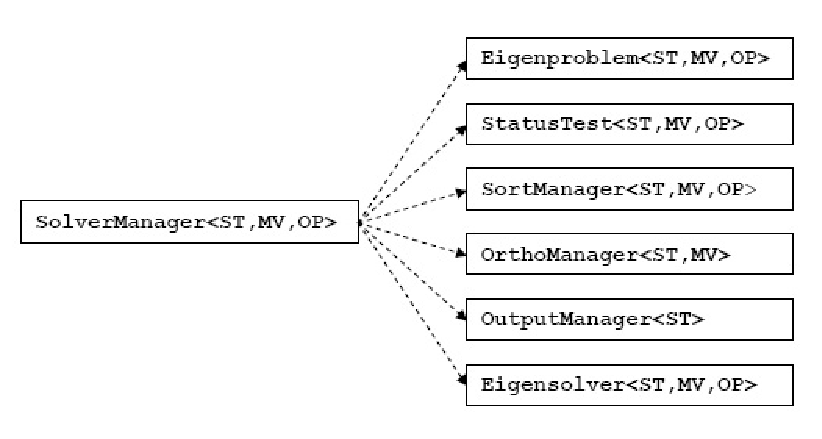
\includegraphics[height=2in]{anasazi_slvr_collaborations.pdf}
\end{center}
\caption{\aspace{SolverManager} class collaboration graph.}
\end{figure}

The first component that is essential to the \aspace{SolverManager} is the
\aspace{Eigenproblem} class.  \aspace {Eigenproblem} is an abstract class that is a
container for the components and solution of an eigenvalue problem. By requiring
eigenvalue problems to derive from \aspace{Eigenproblem}, Anasazi defines a minimum
interface that can be expected of all eigenvalue problems by the classes that will work
with these problems. The methods provided by this interface, shown in Table
\ref{tab:anasazi:eigenproblem}, are generic enough to define an eigenvalue problem that is
standard or generalized, Hermitian or non-Hermitian. Furthermore, this interface allows
the definition of a preconditioner, for preconditioned eigensolvers, as well as the
definition of a spectral transformation, for Arnoldi-based eigensolvers. 

\begin{table}[htb]
\begin{center}
  \caption{A list of methods provided by any derived \aspace{Eigenproblem}.} 
\label{tab:anasazi:eigenproblem}
\begin{tabular}{| p{2cm}  p{2cm} | p{6cm} |}
\hline
\multicolumn{3}{|c|}{\textbf{Eigenproblem$<$ST,MV,OP$>$}} \\\hline
\multicolumn{2}{|c|}{\emph{Method name}} & \emph{Description} \\
\hline
{\tt setOperator()}&{\tt getOperator()}    & Access the operator for which eigenvalues will be computed \\
{\tt setA()}&{\tt getA()}                  & Access the operator A of the eigenvalue problem $Ax=\lambda Mx$  \\
{\tt setM()}&{\tt getM()}                  & Access the operator M of the eigenvalue problem $Ax=\lambda Mx$  \\
{\tt setPrec()}&{\tt getPrec()}            & Access the preconditioner for this eigenvalue problem $Ax=\lambda Mx$  \\
{\tt setInitVec()}&{\tt getInitVec()}      & Access the initial guess \\
{\tt setAuxVecs()}&{\tt getAuxVecs()}      & Access the auxiliary vectors \\
{\tt setNEV()}&{\tt getNEV()}              & Access the number of eigenvalues (NEV) that are requested  \\
{\tt setHermitian()}&{\tt isHermitian()}   & Access the symmetry of the eigenproblem \\
{\tt setProblem()}&{\tt isProblemSet()}    & Access whether the eigenproblem is fully defined  \\
{\tt setSolution()}&{\tt getSolution()}    & Access the solution to the eigenproblem \\
\hline
\end{tabular}
\end{center}
\end{table}

From a user's perspective, the most important part of the interface may be the methods 
for storing and retrieving the results of the eigenvalue computation:
\begin{verbatim}
const Eigensolution & Eigenproblem::getSolution();
void Eigenproblem::setSolution(const Eigensolution & sol);
\end{verbatim}
The \aspace{Eigensolution} class was developed in order to
facilitate setting and retrieving the solution data from an eigenproblem.  
Furthermore, the \aspace{Eigensolution} class was designed for storing
solution data from both Hermitian and non-Hermitian eigenproblems. 
This structure contains the following information:
\begin{itemize}
  \item \verb!RCP<MV> Evecs! \\
   The computed eigenvectors.
 \item \verb!RCP<MV> Espace! \\
   An orthonormal basis for the computed eigenspace.
 \item \verb!std::vector< Value<ST> > Evals! \\
   The computed eigenvalue approximations.
 \item \verb!std::vector<int> index! \\
   An index scheme enabling compressed storage of eigenvectors for non-Hermitian problems.
 \item \verb!int numVecs! \\
   The number of computed eigenpair approximations.
\end{itemize}
The \aspace{Eigensolution::index} vector has \aspace{numVecs} integer entries that take 
one of three values: $\{0, +1, -1\}$. These values allow the eigenvectors to be retrieved as follows:
\begin{itemize}
  \item \aspace{index[i]==0}: The $i$-th eigenvector is stored uncompressed in column $i$ of
    \verb!Evecs!.
  \item \aspace{index[i]==+1}: The $i$-th eigenvector is stored compressed, with the real
    component in column $i$ of \verb!Evecs! and the \emph{positive} complex component
    stored in column $i+1$ of \verb!Evecs!.
  \item \aspace{index[i]==-1}: The $i$-th eigenvector is stored compressed, with the real
    component in column $i-1$ of \verb!Evecs! and the \emph{negative} complex component
    stored in column $i$ of \verb!Evecs!.
\end{itemize}
The compressed storage scheme is necessary to efficiently store the (potentially) complex
eigenvectors of a non-symmetric eigenproblem when the multivectors are defined over a real
field. This scheme enables Anasazi to use \aspace{numVecs} vectors to store
\aspace{numVecs} eigenvectors, even when complex conjugate pairs are present. All other
eigenproblems (real symmetric, complex Hermitian) will return an index vector composed
entirely of zeroes, as compression of complex eigenvectors is not an issue.

%For the real
%non-symmetric case, the $+1$ index will always immediately precede
%the corresponding $-1$ index.

The \aspace{Value} structure is a simple container, templated on scalar type, that
has two members: the real and imaginary part of an eigenvalue.  The real and imaginary
parts are stored as the magnitude type of the scalar type.  The \aspace{Value} structure
along with the \verb!index! vector enable the \aspace{Eigensolution} structure to 
store the solutions from either real or complex, Hermitian or non-Hermitian eigenvalue
problems. Implementations of the \aspace{SolverManager} class are expected to place the 
results of their computation in the \aspace{Eigenproblem} class using an \aspace{Eigensolution}. 

The second component that is essential to a \aspace{SolverManager} is the \aspace{Eigensolver}
class. The \aspace{Eigensolver} abstract base class defines the basic interface that must be met
by any eigen-iteration class in Anasazi. This class defines two types of methods: status methods and
solver-specific methods. A list of these methods is given in Table~\ref{tab:anasazi:itermethods}.
\begin{table}[htp]
\begin{center}
\caption{A list of methods provided by any derived \aspace{Eigensolver}.} 
\label{tab:anasazi:itermethods}
\begin{tabular}{| p{3cm} | p{6cm} |}
\hline
\multicolumn{2}{|c|}{\textbf{Eigensolver$<$ST,MV,OP$>$}} \\\hline
\multicolumn{2}{|c|}{\emph{Status Methods}} \\
\hline
\emph{Method name} & \emph{Description} \\
\hline
{\tt getNumIters()}       & current number of iterations \\
{\tt getRitzValues()}     & most recent Ritz values \\
{\tt getRitzVectors()}    & most recent Ritz vectors \\
{\tt getRitzIndex()}      & Ritz index needed for indexing compressed Ritz vectors \\
{\tt getResNorms()}       & residual norms, with respect to the \aspace{OrthoManager} \\
{\tt getRes2Norms()}      & residual Euclidean norms \\
{\tt getRitzRes2Norms()}  & Ritz residual  Euclidean norms \\
{\tt getCurSubspaceDim()} & current subspace dimension \\
{\tt getMaxSubspaceDim()} & maximum subspace dimension \\
{\tt getBlockSize()}      & block size \\
\hline
\multicolumn{2}{|c|}{\emph{Solver-specific Methods}} \\
\hline
\emph{Method name} & \emph{Description} \\
\hline
{\tt getState()}       & returns a specific structure with read-only pointers to
                       the current state of the solver. \\
{\tt initialize()}     & accepts a solver-specific structure enabling the user to initialize
                       the solver with a particular state.\\
{\tt iterate()}        & performs eigen-iteration until the status test indicates the need
                       to stop or an error occurs.\\
\hline
\end{tabular}
\end{center}
\end{table}
The status methods are defined by the \aspace{Eigensolver}
abstract base class and represent the information about the iteration status that can 
be requested from any eigensolver.  Each eigensolver iteration also provides low-level, 
solver-specific methods for accessing and setting the state of the solver.  
An eigensolver's state is stored in a solver-specific structure and is expected to fully describe 
the current state of the solver or the state the solver needs to be initialized to.  
A simple example of a state structure can be seen in Figure \ref{fig:state}.
\begin{figure}[htb]
\begin{center}
\begin{boxedverbatim}
  template <class ST, class MV>
  struct SomeEigensolverState {
    /* The current dimension of the subspace.                              *
     * NOTE: This should be equal to SomeEigensolver::getCurSubspaceDim(). */
    int curDim;
    /* The current subspace. */
    RCP<const MV> V;
    /* The current Rayleigh-Ritz projection */
    RCP<const Teuchos::SerialDenseMatrix<int,ST> > H;
  };
\end{boxedverbatim}
\end{center}
\caption{Example of an \aspace{Eigensolver} state structure.}
\label{fig:state}
\end{figure}

The eigensolver iterations implemented using the \aspace{Eigensolver} class
are generic iteration kernels that do not have the intelligence to determine when
to stop the iteration, what the eigenvalues of interest are, where to send output,
or how to orthogonalize the basis for a subspace.  The intelligence to perform these four
tasks is, instead, provided by the \aspace{StatusTest}, \aspace{SortManager},
\aspace{OutputManager}, and \aspace{OrthoManager} objects, which are passed into the
constructor of an \aspace{Eigensolver} (Figure \ref{fig:constructor}).  This allows 
each of these four tasks to be modified without affecting the basic eigensolver 
iteration. When combined with the status and state-specific \aspace{Eigensolver} 
methods, this provides the user with a large degree of control over eigensolver iterations.
\begin{figure}[htb]
\begin{center}
\begin{boxedverbatim}
Eigensolver(
   const RCP< Eigenproblem<ST,MV,OP> > &problem,
   const RCP< SortManager<ST,MV,OP>  > &sorter,
   const RCP< OutputManager<ST>      > &printer,
   const RCP< StatusTest<ST,MV,OP>   > &tester,
   const RCP< OrthoManager<ST,OP>    > &ortho,
   ParameterList                       &params
 );
\end{boxedverbatim}
\end{center}
\caption{Basic constructor for an \aspace{Eigensolver}}
\label{fig:constructor}
\end{figure}

The abstract \aspace{StatusTest} class is used to provide the interface for stopping 
conditions for an eigen-iteration. There are numerous conditions under which an eigen-iteration 
should be stopped, with the most common conditions being the number of iterations,
convergence criterion, and deflation of converged eigenpairs.
Often the decision to stop an eigensolver iteration is based on a hierarchy 
of problem-dependent, logically connected stopping conditions.
This, possibly complex, reasoning should not be encoded in the \aspace{Eigensolver} class,
which instead queries the \aspace{StatusTest} during its class method \aspace{iterate()} to determine 
whether or not to continue iterating (Figure~\ref{fig:comm}).
\begin{figure}[htb]
\begin{center}
\begin{boxedverbatim}
SomeEigensolver::iterate() {
  while ( somestatustest.checkStatus(this) != Passed ) {
    //
    // perform eigensolver iterations
    //
  }
  return;  // return back to caller
}
\end{boxedverbatim}
\end{center}
\caption{Example of communication between status test and eigensolver}
\label{fig:comm}
\end{figure}
The \aspace{StatusTest} class provides a method, \verb!checkStatus()!, which queries the methods provided by
\aspace{Eigensolver} and determines whether the solver meets the criteria defined by the 
status test. After a solver returns from \verb!iterate()!, the caller has the ability to access the
solver's state and the option to re-initialize the solver with a new state and continue
the iteration.

A \aspace{StatusTest} is a desirable feature in the Anasazi software framework because it
provides the eigensolver user and developer with a flexible interface for interrogating
the eigen-iteration. Besides the basic usage, this interface makes it possible to, for
example, select stopping conditions at runtime or put application-specific hooks in the
eigensolver for debugging and checkpointing. This flexible approach to selecting and
developing stopping criteria for an eigensolver is not available in PRIMME or SLEPc.
Since an ARPACK user provides the memory for computations and ARPACK is constantly
returning control via the reverse communication mechanism, the user has some ability to
examine the current state and modify it to force certain behavior. However, this is an
advanced use case which requires intimacy with the formatting of the ARPACK control data.

The purpose of the \aspace{SortManager} class is to separate the \aspace{Eigensolver} from
the sorting functionality, giving users the opportunity to choose the eigenvalues of
interest in whatever manner is deemed to be most appropriate. Anasazi defines an abstract
class \aspace{SortManager} with two methods, one for sorting real values and one for
sorting complex values, shown in Figure \ref{fig:sort}.  The \aspace{SortManager} is also
expected to provide the permutation vector if the \aspace{Eigensolver} passes a non-null
pointer for \verb!perm! to the \aspace{sort} method.  This is necessary, because many
eigen-iterations must sort their approximate eigenvectors, as well as their eigenvalues.

\begin{figure}[htb]
\begin{center}
\begin{boxedverbatim}
// Sort n real values stored in evals and return permutation, if required, in perm.
void sort(Eigensolver<ST,MV,OP>* solver, 
          const int n, 
          std::vector<typename Teuchos::ScalarTraits<ST>::magnitudeType> &evals,
          std::vector<int> *perm) 
// Sort n complex values, whose real and imaginary part are stored in r_evals 
//   and i_evals, respectively. Return permutation, if required, in perm.
void sort(Eigensolver<ST,MV,OP>* solver, 
          const int n, 
          std::vector<typename Teuchos::ScalarTraits<ST>::magnitudeType> &r_evals, 
          std::vector<typename Teuchos::ScalarTraits<ST>::magnitudeType> &i_evals, 
          std::vector<int> *perm)
\end{boxedverbatim}
\end{center}
\caption{A list of methods provided by any derived \aspace{SortManager}.} \label{fig:sort}
\end{figure}

Since orthogonalization and orthonormalization are commonly performed
computations in iterative eigensolvers and can be implemented in a variety of ways, 
the \aspace{OrthoManager} class separates the \aspace{Eigensolver}
from this functionality. The \aspace{OrthoManager} defines a small number of
orthogonalization-related operations, including a choice of an inner
product, which are listed in Table \ref{tab:anasazi:orthomanager}.  The \aspace{OrthoManager} interface
\begin{table}[htp]
\begin{center}
\caption{A list of methods provided by any derived \aspace{OrthoManager}.} 
\label{tab:anasazi:orthomanager}
\begin{tabular}{| p{4cm} | p{6cm} |}
\hline
\multicolumn{2}{|c|}{\textbf{OrthoManager$<$ST,MV$>$}} \\\hline
\emph{Method name} & \emph{Description} \\
\hline
{\tt innerProd(X,Y,Z)} &
Provides the inner product defining the concepts of orthogonality: $Z = \langle X, Y \rangle$ \\
{\tt norm(X,normvec)} &
Provides the norm norm induced by the inner product: $normvec[i] = \sqrt{\langle X[i], Y[i] \rangle}$\\
{\tt project(X,Q,C) } &
Projects the multivector X onto the subspace orthogonal to the multivectors Q, optionally returning the coefficients of 
X with respect to the Q.\\
{\tt normalize(X,B)} &
Computes an orthonormal basis for the multivector X, optionally returning the coefficients
of X with respect to the computed basis.\\
{\tt projectAndNormalize(X,Q,C,B)} &
Projects the multivector X onto the subspace orthogonal to the multivectors Q and computes an orthonormal basis (orthogonal to the Q) 
for the resultant, optionally returning the coefficients of X with respect to the Q and the computed basis.\\
\hline
\end{tabular}
\end{center}
\end{table}
has also been extended, through inheritance, to support orthogonalization and 
orthonormalization using matrix-based inner products in the \aspace{MatOrthoManager}
class. This extended interface allows the eigen-iteration to pass in pre-computed
matrix-vector products that can be used in the orthogonalization and orthonormalization
process, thus making the computation more efficient.

The \aspace{Eigensolver} class combined with the utilities provided by the \aspace{StatusTest},
\aspace{SortManager}, and \aspace{OrthoManager} classes provides a powerful, flexible way
to design an eigen-iteration.  However, directly interfacing with the \aspace{Eigensolver} class
can be overwhelming, since it requires the user to construct a number of support classes and 
manage calls to \verb!Eigensolver::iterate()!. The \aspace{SolverManager} class was developed to
encapsulate an instantiation of \aspace{Eigensolver}, providing additional functionality
and handling low-level interaction with the eigensolver iteration that a user may not want to
specify. 

Solver managers are intended to be easy to use, while still providing the
features and flexibility needed to solve large-scale eigenvalue problems.
The \aspace{SolverManager} constructor accepts only two arguments:
an \aspace{Eigenproblem} specifying the eigenvalue problem to be solved and a
\texttt{ParameterList} of options specific to this solver manager. 
\begin{figure}[htb]
\begin{center}
\begin{boxedverbatim}
SolverManager(
   const RCP< Eigenproblem<ST,MV,OP> > &problem,
   ParameterList                       &params
 );
\end{boxedverbatim}
\end{center}
\caption{Basic constructor for a \aspace{SolverManager}}
\label{fig:constructor2}
\end{figure}
The solver manager instantiates an \aspace{Eigensolver} implementation, along with the
status tests and other support classes needed by the eigensolver iteration, as
specified by the parameter list. To solve the eigenvalue
problem, the user simply calls the \verb!solve()! method of the \aspace{SolverManager},
which returns either \aspace{Converged} or \aspace{Unconverged}, and retrieves the computed
\aspace{Eigensolution} from the \aspace{Eigenproblem} (Figure \ref{fig:examplesolve}).

\begin{figure}[htb]
\begin{center}
\begin{boxedverbatim}
// create an eigenproblem
RCP< Anasazi::Eigenproblem<ST,MV,OP> > problem = ...;
// create a parameter list
ParameterList params;
params.set(...);
// create a solver manager
Anasazi::SolverManager<ST,MV,OP> solman(problem,params);
// solve the eigenvalue problem
Anasazi::ReturnType ret = solman.solve();
// get the solution from the problem
Anasazi::Eigensolution<ST,MV> sol = problem->getSolution();
\end{boxedverbatim}
\end{center}
\caption{Sample code for solving an eigenvalue problem using a \aspace{SolverManager}}
\label{fig:examplesolve}
\end{figure}

The simplicity of the \aspace{SolverManager} interface often conceals a complex eigensolver strategy.
The purpose of many solver managers is to manage and initiate the repeated calls to the underlying 
\aspace{Eigensolver::iterate()} method. For
solvers that increase the dimension of trial and test subspaces (e.g., Davidson and Krylov
subspace methods), the solver manager may also assume the task of restarting (so that
storage costs may be fixed). This decoupling of restarting from the eigensolver is
beneficial due to the numerous restarting techniques in use.

Under this framework, users have a number of options for performing eigenvalue
computations with Anasazi:
\begin{itemize}
\item
Use the existing solver managers, which we will discuss in the next section. 
In this case, the user is limited to the functionality provided by the existing 
solver managers.
\item
Develop a new solver manager for an existing eigensolver iteration.
The user can extend the functionality provided by the eigen-iteration,
specifying custom configurations for status tests, orthogonalization, restarting, 
locking, etc.
\item
Implement a new eigensolver iteration, thus taking advantage of Anasazi's extensibility. 
The user can write an eigensolver iteration that is not provided by Anasazi. 
The user still has the benefit of the available support classes 
and the knowledge that this effort can be easily employed by anyone already 
familiar with Anasazi.
\end{itemize}
In the next section we will discuss the current implementations of
eigensolver iterations and managers, as well as utility classes, provided
by the Anasazi eigensolver framework.

\subsection{Anasazi Class Implementations}
%%%%%%%%%%%%%%%%%%%%%%%%%%%%%%%%%%%%%%%%%%%%%%%%%%%%%%
\label{subsec:anasazi:classes}

Anasazi is an eigensolver software framework designed with extensibility in mind, 
so that users can augment the package with any special functionality that may be
needed. However, the released version of Anasazi provides all
functionality necessary for solving a wide variety of problems. This
section lists and briefly describes the class implementations provided
by Anasazi.

\subsubsection{\aspace{Anasazi::Eigenproblem}}

Anasazi provides users with a concrete implementation of
\aspace{Eigenproblem}, called \aspace{BasicEigenproblem}. This basic implementation
provides all the functionality necessary to describe both generalized and standard,
Hermitian and non-Hermitian linear eigenvalue problems. This implementation fully 
supports the definition of a preconditioner, for preconditioned eigensolvers, 
as well as the definition of a spectral transformation, for Arnoldi-based eigensolvers. 

\subsubsection{\aspace{Anasazi::Eigensolver}}

Anasazi provides users with a concrete implementation of three popular algorithms:
\begin{enumerate}
  \item a block extension of a Krylov-Schur method~\cite{stew:01},
  \item a block Davidson method as described in~\cite{Arbenz:2005:ACE},
  \item an implementation of LOBPCG as described in~\cite{Hetmaniuk:2006:BSL}.
\end{enumerate}
These implementations can be found in the \aspace{BlockKrylovSchur}, \aspace{BlockDavidson}, 
and \aspace{LOBPCG} classes, respectively. Only the block Krylov-Schur method can be used
for non-Hermitian generalized eigenvalue problems. In contrast, all three algorithms can 
be used for symmetric positive semi-definite generalized eigenvalue problems.

\subsubsection{\aspace{Anasazi::StatusTest}}

The purpose of the \aspace{StatusTest} is to give the user or solver
manager flexibility in terminating the eigensolver iterations in
order to interact directly with the solver. Typical
reasons for terminating the iteration are:
\begin{itemize}
  \item some convergence criterion has been satisfied;
  \item some portion of the subspace has reached sufficient accuracy to be
  deflated from the iterate or locked;
  \item the solver has performed a sufficient number of iterations.
\end{itemize}
With respect to these reasons, the following is a list of Anasazi-provided status tests:
\begin{itemize}
  \item \aspace{StatusTestMaxIters} - monitors the number of iterations
    performed by the solver; it can be used to halt the solver at some maximum number of iterations
    or even to require some minimum number of iterations.
  \item \aspace{StatusTestResNorm} - monitors the residual norms of the
    current iterate.
  \item \aspace{StatusTestCombo} - a boolean combination of
    other status tests, creating unlimited potential for complex status tests.
  \item \aspace{StatusTestOutput} - a wrapper around another
    status test, allowing for printing of status information on a call to
    \verb!checkStatus()!.
\end{itemize}

\subsubsection{\aspace{Anasazi::SortManager}}

The purpose of the \aspace{SortManager} is to give users the opportunity to choose the 
eigenvalues of interest in whatever manner is deemed to be most appropriate. 
Typically, the eigenvalues of interest are those with:
\begin{itemize}
  \item the smallest or largest magnitude
  \item the smallest or largest real part
  \item the smallest or largest imaginary part
\end{itemize}
Anasazi provides the ability to perform these six sorts in the \aspace{BasicSortManager}
class. Other implementations of \aspace{SortManager} may, for example, be tailored to
account for the effects of chosen spectral transformations.

\subsubsection{\aspace{Anasazi::OrthoManager}}

The eigen-iteration implementations provided by Anasazi are all orthogonal 
Rayleigh-Ritz methods where an orthonormal basis representation is computed. 
Motivated by the plethora of available methods for performing these 
computations, Anasazi has left as much leeway to the users as possible. 
Anasazi provides two concrete orthogonalization managers:
\begin{itemize}
\item
  \aspace{BasicOrthoManager} - performs orthogonalization using
  classical Gram-Schmidt with a possible DGKS correction step~\cite{dgks:76}
\item
  \aspace{SVQBOrthoManager} - performs orthogonalization using the
  SVQB orthogonalization technique described by Stathapoulos and
  Wu~\cite{Stathopoulos:2002:BOP}
\end{itemize}


%When solving real symmetric eigenproblems, the eigenvectors can always
%be chosen to be real, and therefore can be stored in a single column
%of a real multivector. When solving eigenproblems over a complex
%field, whether Hermitian or non-Hermitian, the eigenvectors may be
%complex, but the multivector is defined over the complex field, so
%that this poses no problem. However, real non-symmetric problems can
%have complex eigenvectors, which prohibits a one-for-one storage
%scheme using a real multivector.  Fortunately, the eigenvectors in
%this scenario occur as complex conjugate pairs, so the pair can be
%stored in two real vectors. This permits a compressed storage scheme,
%which uses an index vector stored in the \aspace{Eigensolution},
%allowing conjugate pair eigenvectors to be easily retrieved from
%\verb!Evecs!.

%\begin{remark}
%  Solver managers all put the computed eigensolution into the eigenproblem class before
%  returning from \verb!solve()!. Eigensolvers do not; a user working directly with an
%  eigensolver will need to recover the solution directly from the eigensolver state.
%\end{remark}


% powerful, but can be tedious. Solver managers provide a way for users
% to encapsulate specific solving strategies inside of an easy-to-use
% class. Novice users may prefer to use existing solver managers, while
% advanced user may prefer to write custom solver managers.

\subsubsection{\aspace{Anasazi::SolverManager}}

Anasazi provides at least one solver manager for each implemented eigensolver iteration:
\begin{itemize}
  \item \aspace{BlockKrylovSchurSolMgr} - provides a solver manager for the
    \aspace{BlockKrylovSchur} eigensolver with restarting.
  When the block size is one, this Krylov-subspace method is mathematically equivalent to the
  implicitly-restarted Arnoldi method in ARPACK. 
  \item \aspace{BlockDavidsonSolMgr} - provides a solver manager for the
    \aspace{BlockDavidson} eigensolver which performs restarts and locking/deflating of
    converged eigenvectors.
  \item \aspace{LOBPCGSolMgr} - provides a solver manager for the \aspace{LOBPCG}
    eigensolver which provides a lock/deflating mechanism for converged eigenvectors.
  \item \aspace{SimpleLOBPCGSolMgr} - a simple solver manager for the \space{LOBPCG}
    eigensolver, providing a checkpointing eigensolver. This solver manager is intended
    as an example of how a solver manager should be constructed.
\end{itemize}

%All of these solver managers are constructed using an \aspace{Eigenproblem} and a 
%solver-specific \aspace{ParameterList}, and have a \verb!solve()! method that takes no
%arguments and returns either \aspace{Converged} or \aspace{Unconverged}. Figure~\ref{fig:examplesolve}
%provides a sample code that creates an \aspace{Eigenproblem} and \aspace{ParameterList}, uses it 
%to create a \aspace{SolverManager}, solves the eigenproblem, and retrieves the \aspace{Eigensolution}.

% These examples are meant to illustrate the flexibility that specific
% solver managers may have in implementing the \verb!solve()! routine.
% Some of these options might best be incorporated into a single
% solver manager, which takes orders from the user via the parameter
% list given in the constructor. Some of these options may better be
% contained in multiple solver managers, for the sake of code
% simplicity. It is even possible to write solver managers that
% contain other solvers managers; motivation for something like this
% would be to select the optimal solver manager at runtime based on
% some expert knowledge, or to create a hybrid method which uses the
% output from one solver manager to initialize another one.

%Anasazi
%provides a concrete implementation called \aspace{BasicSort}.  This class provides basic
%functionality for selecting significant eigenvalues: by largest or smallest real part, by
%largest or smallest imaginary part, or by largest or smallest magnitude.

\section{Benchmarking}
%%%%%%%%%%%%%%%%%%%%%%%%%%%%%%%%%%%%%%%%%%%%%%%%%%%%%%
\label{sec:benchmarking}

The benefits of an object-oriented eigensolver framework such as Anasazi are many:
modularization provides improved code reuse, static polymorphism via templating allows
easier code maintenance and a larger audience through software interoperability, and
dynamic polymorphism via inheritance allows easy extension of capability and flexible
runtime behavior. However, none of these benefits should come at the expense of code
performance. Concern over overhead has long been an inhibiting factor in the adoption of
object-oriented programming paradigms in scientific computing. In this section we 
address this important issue by comparing Anasazi and ARPACK on a model problem. Our
interest is in addressing concerns about the overhead of Anasazi and ARPACK, C++ and
FORTRAN 77 software.

We compared Anasazi's \aspace{BlockKrylovSchurSolMgr} (with a block size
of one) and ARPACK's \aspace{dnaupd}, which each compute approximations to the
eigenspace of a non-symmetric matrix. Our goal was to benchmark the
cost of computing $50, 100, 150$ Arnoldi vectors for a finite
difference approximation to a two dimensional convection diffusion
problem. Both codes use classical Gram-Schmidt with the DGKS \cite{dgks:76} 
correction for maintaining the numerical orthogonality of the Arnoldi basis
vectors.  The Intel 9.1 C++ and FORTRAN compilers were used with
compiler switches ``-O2 -xP'' on an Intel Pentium D, 3GHz, 1MB L2
cache, 2GB main, Linux/FC5 PC.  The results of this study can be found
in Table~\ref{table:timings}.

\begin{table}
\caption{Illustrating the overhead of Anasazi as compared to ARPACK; ``---'' denotes a measurement
below the clock resolution. Each timing is the average over three runs.}
\label{table:timings}
\begin{center}
\begin{tabular}{r|ll|ll|}
       \cline{2-5} %\hline
       % after \\: \hline or \cline{col1-col2} \cline{col3-col4} ...
        & \multicolumn{4}{c|}{Computing $50$ Arnoldi vectors} \\ \cline{2-5}
        & \multicolumn{2}{c|}{Matrix-vector time [s]} &
       \multicolumn{2}{c|}{Total runtime [s]}\\ \hline
       Matrix size & ARPACK & Anasazi & ARPACK & Anasazi \\ \hline %\cline{2-5}
       %2500 & 0.010 & 0.018 & 0.47 & 0.54 \\
       10000 & --- & 0.01 & 0.14 & 0.15 \\
       62500 & 0.04 & 0.09 & 1.20 & 1.17 \\
       250000 & 0.15 & 0.32 & 4.98 & 4.79 \\
       1000000 & 0.66 & 1.23 & 19.2 & 18.8 \\
       \hline
        & \multicolumn{4}{c|}{Computing $100$ Arnoldi vectors} \\ \cline{2-5}
        & \multicolumn{2}{c|}{Matrix-vector time [s]} &
       \multicolumn{2}{c|}{Total runtime [s]}\\ \hline
       Matrix size & ARPACK & Anasazi & ARPACK & Anasazi \\ \hline %\cline{2-5}
       %2500 & 0.010 & 0.018 & 0.47 & 0.54 \\
       10000 & 0.03 & 0.02 & 0.53 & 0.55 \\
       62500 & 0.03 & 0.17 & 4.37 & 4.29 \\
       250000 & 0.34 & 0.64 & 17.8 & 17.5 \\
       1000000 & 1.27 & 2.40 & 68.4 & 67.1 \\
       \hline
        & \multicolumn{4}{c|}{Computing $150$ Arnoldi vectors} \\ \cline{2-5}
        & \multicolumn{2}{c|}{Matrix-vector time [s]} &
       \multicolumn{2}{c|}{Total runtime [s]}\\ \hline
       Matrix size & ARPACK & Anasazi & ARPACK & Anasazi \\ \hline %\cline{2-5}
       %2500 & 0.010 & 0.018 & 0.47 & 0.54 \\
       10000 & 0.03 & 0.04 & 1.15 & 1.22 \\
       62500 & 0.14 & 0.26 & 9.53 & 9.39 \\
       250000 & 0.50 & 0.96 & 38.1 & 38.0 \\
       1000000 & 1.97 & 3.56 & 149 & 146 \\
       \hline
     \end{tabular}
\end{center}
\end{table}

The operator application in Anasazi records approximately twice as much time as the ARPACK
implementation. This is because the Anasazi code used an Epetra sparse matrix
representation for the linear operator, while the ARPACK implementation applies the block
tridiagonal matrix via a stencil (which would have been possible via a different choice of
operator). Note that the operator application comprised only a small portion of the clock
time in these tests. The majority of the clock time was consumed via the orthogonalization
routines which support the Arnoldi iteration. It should be noted that while these routines
are hard-coded in the ARPACK FORTRAN 77 library, they are accessed through a dynamic
polymorphic interface in Anasazi. Regardless, the performance of the Anasazi library in
computing the Arnoldi vectors is similar to that of ARPACK. This illustrates that a
well-designed library in C++ can be as efficient as a FORTRAN 77 library.

\section{Conclusion}

We believe that Anasazi is the natural successor to ARPACK, inheriting and extending the
quality practices employed by ARPACK. Anasazi takes advantage of the generic and
object-oriented language features of C++, allowing it to improve on the design of related
eigensolver efforts. The use of static polymorphism via templated code replaces the
reverse communication model which helped to popularize ARPACK and enable its adoption as
the default eigensolver in many scientific communities. The decoupling of algorithmic
components, via dynamic polymorphism, is beneficial from a software engineering point of
view, by easing component verification, enabling code reuse, and maximizing runtime
flexibility in implementation. Furthermore, this decoupling allows Anasazi to act as a
research platform not only for eigensolvers, but also for those components which are vital
to the efficient and effective implementation of large-scale eigensolvers.


\section{Acknowledgments}

We thank Roscoe Bartlett, Mike Heroux, Roger Pawlowski, Eric Phipps, and Andy Salinger for
many helpful discussions. We appreciate the suggestions and corrections of the anonymous
reviewers.

\bibliography{anasazi-toms}
\bibliographystyle{acmtrans}


\begin{received}
%????
\end{received}


\end{document}
